\chapter{イントロダクション}
\section{太陽運動・銀河回転パラメータ決定の現状・課題}
% * 1.1 歴史的流れ ← 適切なタイトルに変える
% せっかく書いてくれましたが、ちょっとMilky Wayの発見までの
% 歴史的流れが長いかなぁ、という印象です。
% それに対して、今回の修論の主題に関わる内容の
% 歴史的な流れ (LindbladやOortのこと) の分量が少ないですね。。
% Oortの後に、チャンドラセカールによる一般化が続くと思います。

% 天の川銀河が円盤状の形をして回転していることがわかったのは、最近200年のことである。18世紀にウィリアム・ハーシェル (William Herschel) は600以上の異なる場所で空を観測し、全ての星が同じ輝度を持ち、地球からの各星までの距離を見積もることができると仮定した。彼はこのデータを使って数えた星と地球からの距離を組み込んだ空全体の地図を作成した (図\ref{Herschel})。
% \begin{figure*}[htbp]
% \begin{center}
% 	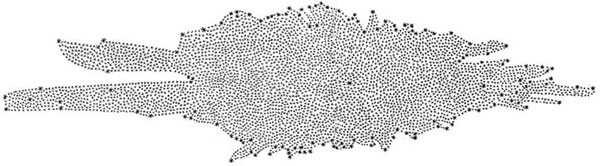
\includegraphics[width=8cm]{fig/Herschel.jpg}
% 	\caption{天の川のさまざまな部分の星の数を数えたことから導かれた天の川の地図 (\cite{Herschel1785})。中心付近に位置する黒い点が太陽を表している。}
% 	\label{Herschel}
% \end{center}
% \end{figure*}
% 彼はこの研究から、太陽は天の川の中心あるいは中心付近に位置しているという結論を出した。また、ハーシェルの示した恒星の分布は、直径約2 kpc、厚さ約400 pcほどのものであった。その後、20世紀初頭にカプタイン (Jacobus Kapteyn) は世界中の天文学者の助けを借りてハーシェルの天の川の地図よりも高精度な地図を作成した。カプタインが示した天の川は、直径約17 kpc、厚さ約3 kpcというものであった。しかし、カプタインもまた太陽は天の川の中心に位置していると考えていた。その理由は、実際には銀河中心に星が密集しているが、星間塵による星の光の強い星間吸収の影響でよく見えず、その結果どの方向でも星は同じように分布しているように見えるためである。

% 1920年、シャプレー (Harlow Shapley) によって、銀河系中心という特別な場所に太陽が位置するという理論を覆された。彼は最も近い球状星団に含まれること座RR型変光星を観測し、年周視差と変光星の周期-光度関係を利用することでその星団までの距離を測定した。同様に変光星を利用していくつかの球状星団の天球面上の位置と距離を決定していくと、銀河系の全体像が浮かび上がった。すると、彼は球状星団が射手座の方向のある一点の周囲に球状に分布していることを発見した。その後、その点を銀河系の中心として提案し、太陽は銀河系の中心から離れた場所に位置していることを示した。この発見は地動説に次ぐ天文学上の最も重要な発見である。

%太陽系は現時点では生命が存在することが確認されている唯一の惑星系である。太陽系は約46億年の歴史の中で、誕生から22回ほど銀河中心の周りを回転してきたと考えられる (\cite{Adams2010})。太陽系の起源と誕生からの歴史を決定することは、太陽系に生命が誕生し、生存を続けている理由を明らかにする方法の1つとなる。力学的なアプローチとしては、太陽系を含めた恒星系の回転運動を決めることが必要不可欠となる。太陽運動とオールト定数を決定することは太陽系が描いてきた軌道を知るための重要な方法の1つである。太陽系の軌道を決定できれば、太陽系がどのような環境で生まれ、どのような歴史を辿ってきたのかが分かれば、太陽系のような惑星系の形成に制限をつけられる可能性がある。

天の川銀河円盤は自己重力による重力ポテンシャルから受ける中心力と回転による遠心力とがつり合って回転を続けられている。つまり、銀河系の各半径での天体の回転運動は質量分布を反映したものとなる。したがって、銀河系円盤の回転運動の様子を理解することは、天の川銀河の動力学を理解する上で非常に重要である。さらに、銀河系内での太陽系の運動を調べることは、太陽系がどこで生まれたかを知るヒントとなる上、銀河系内の力学構造を解釈するためには天体が銀河系中心に対してどのような速度で動いているのかを知る必要があるため、観測した天体の運動速度に対して太陽系の運動速度で補正する形で用いる必要があることから、位置天文学や銀河動力学において主要な課題の1つとなっている。

天の川銀河が回転していることが定着したのは天文学の長い歴史の中でもこの100年のことである。1926年、リンドブラッド  (Bertil Lindblad) はカプタイン (Jacobus Kapteyn) によって20世紀初頭に研究された恒星の運動の様子は銀河系回転によるものあると説明した。彼は、銀河中心に近い星は銀河中心から離れた星よりも速く回転することを提案した。その後オールト (Jan Oort) は、多くの星の速度を観察して1927年にリンドブラッドの理論を証明し、さらにその理論を修正した。彼はオールト定数$A,B$を導入し、銀河系が差動回転していることを示した。また、オールトは太陽系が銀河中心から約10 kpcの距離に位置していると計算した。これらの研究により、太陽系は天の川銀河の円盤の中を他の星と共に回転している描像が明らかとなった。

太陽近傍の星の運動は系統 (平均) 運動にランダム運動 (特異運動) を足したものとして解釈される。円盤銀河では、系統運動が特異運動に比べて支配的である。そのような恒星系は力学的に冷たいと言われる。すなわち、特異運動が系統運動に対して無視できるような系である。例えば、太陽近傍では円盤面の速度分散すなわち特異運動の大きさは古い星の恒星円盤では\SI{45}{km.s^{-1}}、誕生初期の星では\SI{18}{km.s^{-1}}である一方、系統運動は\SI{200}{km.s^{-1}}のオーダーである。特異運動が消える力学的に冷たい極限では、系統運動は重力ポテンシャルによって生まれる閉じた軌道に沿ったものになる。したがって、銀河系回転は重力ポテンシャルから受ける中心力と遠心力とのつり合い、すなわち回転平衡によ
って支えられていることから、天の川銀河のポテンシャルと質量分布は恒星系の系統運動から得ることができる。

\cite{Oort1927a}は、銀河系円盤を回転している天体が閉じた軌道を描いている、すなわち銀河系円盤は力学的に冷たい系であると仮定し、太陽近傍星の位置・速度の観測量を銀河系回転パラメータ$A,B$で記述するモデルを考えた。この$A、B$はいわゆるオールト定数であり、それぞれ銀河回転方向の剪断成分、回転成分を表す。\cite{Chandra42}は、オールトのこのモデルを銀河系円盤の持つ非対称な系統運動の速度場にも適用できるように拡張し、新たな定数$C,K$を導入した。$C、K$はそれぞれ動径方向の剪断成分、発散成分を表す。本論文では、彼らによって構築されたモデルをOort-Lindbladモデル、またこのモデルによる解析をオールト解析と呼ぶことにする (\cite{Oort1927a},\cite{Lindblad1927},\cite{Chandra42})。

% 研究のIntroduction (研究背景・基本事項)、定性的に書く (定量的な事は2章で)
% あと最後に、先行研究 (Olling & Dehnen 2002; Bovy 2017; Vickers & Smith 2018など) で
% 何がどこまでわかっていて、何がわかっていないのかを書いて、
% それを踏まえて、今回の修論の研究のポイントとの違いをしっかり書かないとダメです。
% これが「研究動機」になるはずです。

% * 1.2 現状・課題 ← 適切なタイトルに変える
% 前のセクションでは銀河回転 (オールト定数) の話だったので、
% それに関する「現状・課題」を書いてあるのかと思ったら、
% 急に「太陽運動」の話になっていて、これでは「現状・課題」ではないと思います。
% また「現状」については、書いてあるように見えますが 
% (本当はもっと最近の研究まで書いたほうがよいですが)、
% 「課題」が明確に書かれていない印象です。

これまで、いくつかの先行研究によって太陽運動 (太陽の特異運動) と銀河系速度場パラメータ (オールト定数) が求められてきた。太陽系近傍の銀河系回転運動の測定には星や星間ガスの位置と速度の情報が用いられるが、簡単ではない。星は速度分散が大きい一方、星間ガスは距離測定が難しいという問題がある。本論文では星に対してオールト解析を行うが、先述の通りOort-Lindbladモデルは力学的に非常に冷たい系、すなわち速度分散が回転運動に比べて非常に小さく無視できるような系を仮定したモデルである。しかし、実際に天の川銀河円盤は無視できない程度の速度分散を持っており、解析においては速度分散を考慮しなくてはならない。また、セファイドやOB型星など非常に若い、かつ重い星は質量が重く誕生から間もないことから速度分散は小さいと考えられるが、サンプル数が少なかったり、運動集団や分子雲の運動情報を保っているために平均速度が大きくずれることで、その位置での重力ポテンシャルを表していない可能性がある。

表\ref{table2},\ref{table3}、図\ref{fig:uvw}は先行研究で得られた太陽運動とオールト定数の値である。\cite{Delhaye1965}は異なるスペクトル型と光度の集団を調べることによって太陽運動を$(U_{\odot},V_{\odot},W_{\odot})=(9,12,7)$\,\si{km.s^{-1}}程度とした。これは3つとも現在でも使用される値である。ここで、$(U_{\odot},V_{\odot},W_{\odot})$はそれぞれ太陽から銀河中心に向かう方向、太陽の銀河回転方向かつ$U_{\odot}$に垂直な方向、銀北極方向のLSRに対する太陽の速度である。ヒッパルコス衛星が打ち上がる以前は、長い間\cite{Delhaye1965}の値が主に使われた。\cite{DB1998}はStr\"{o}mbergのasymmetric drift関係を用いることで$Hipparcos$のデータから$(U_{\odot},V_{\odot},W_{\odot}) = (10.0, 5.2, 7.2)\,\si{km.s^{-1}}$ と測定した。

asymmetric driftとは、星の銀河回転速度が、その星の周りの星の集団の速度分散の動径方向成分の大きさにだいたい比例して星の集団の銀河回転速度が遅くなる現象のことである。詳しくは\ref{sec_AD}で説明する。

$U_{\odot}, W_{\odot}$については\cite{DB1998}の30年以上前に導かれたDelhayeの値とほぼ同じ値となっている。$V_{\odot}$については後にDelhayeの値と近い値に修正された(\cite{Schonrich2010})。\cite{OD03}は、ACT/Tycho-2カタログから10万個の11等級より明るい星のデータを用いて、assymetric driftとmode mixingを考慮して解析することでオールト定数を求めた。\cite{Bovy17}ではGaia Data Release 1 (DR1) から約30万個の主系列星を用いて速度場パラメータを測定した。ただし、彼らは視線速度のデータを用いておらず、正確なパラメータ測定ができていない可能性がある。\cite{VS18}はTycho-$Gaia$ Astrometric Solution (TGAS; \cite{Gaia2016}) とRAVE、LAMOSTをクロスマッチさせ、約12万個の星を使用して、年齢推定と銀河系速度場パラメータの測定を行った。しかし、彼らは太陽運動を仮定して解析しており、太陽運動の値は得ていない。

現状の太陽運動解析における最大の問題点は、Oort-Lindbladモデルの仮定に最適なサンプルを選ぼうとする際に、一長一短があるということである。若い星のサンプルを用いれば速度分散は小さいが、運動集団などによって平均速度が銀河ポテンシャルを正確に反映していなかったり、サンプル数が足りなかったりする。一方、古い星はその平均速度が銀河ポテンシャルを反映するものの、速度分散が非常に大きくOort-Lindbladモデルの仮定から大きく逸脱してしまうという問題がある。\cite{OD03}はこれらの問題点を丁寧に扱ったが、彼らの解析では視線速度を用いておらず、またオールト定数のみの測定をしており、太陽運動の値は\cite{OD03}で決定された値を仮定して解析している。

また、もう1つの問題点として、銀河系中心に対する太陽系の運動の値によって他のパラメータが変化してしまうことから、独立に測定すればいいものではないという問題がある。つまり、観測した速度はあくまで太陽から見たときの相対速度であり、銀河系中心を基準としたときの運動に変換するためには太陽運動を仮定する必要がある。また、逆に周りの星の運動速度によって太陽運動の測定値も変化する。このように太陽運動とオールト定数はそれぞれが影響し合うパラメータとなっていることから、別々に測定することは原理上好ましくない。

さらに、asymmetric driftの効果が実際どの程度存在するのかを評価する必要がある。なぜなら、観測データで解析をする際にasymmetric driftを考慮しても、その解析結果の値が正しいのかが分からないからである。しかし、asymmetric driftの効果の定量的な評価はまだ行われておらず、asymmetric driftを考慮せず解析する際にどの程度本当の値から間違えるのかを評価する必要がある。

\section{本研究の目的・本論文の流れ}
% * 1.3 研究動機 → 本研究の動機
% ここの最初に「課題」っぽいことが書かれているように見えますね。。

% 論文の書き方の本などを見て、研究背景 or イントロダクションで書く、
% 先行研究 (これまでの研究の流れ)・先行研究の課題点・研究動機
% をどう書くべきか、もっと考えてみてください。

%先述のように、太陽系の起源と誕生からの歴史を決定することは、太陽系に生命が誕生し、生存を続けている理由を明らかにする方法の1つとなる。例えば、太陽系の銀河中心周りの円運動速度が$v_{\mathrm{c}}$であるとする。また、太陽系の軌道の速度と銀河中心との距離$R_{\mathrm{g}}$は一定であるとする。このとき、太陽系が誕生してから現在までの期間$t$の間の銀河中心周りの回転数は$N_{\mathrm{orb}}=(v_{\mathrm{c}}t)/(2\pi R_{\mathrm{g}})$と書ける。このとき、$v_{\mathrm{c}}$の値が$2$だけ異なるとすると、回転数は約0.2回転だけ変化する。これは銀河中心に対する角度にして$72$度となり、軌道の距離にして約$10\,\mathrm{kpc}$のずれとなる。これは太陽系の誕生環境を考える上で、決して高い精度ではないと考える。

以上の問題点を踏まえ、本研究では2018年4月に公開されたGaia Data Release 2 (DR2) から視線速度を含めた6次元位相空間データ (位置・速度の6次元) を用いて運動学的性質を考慮してできる限り正確な太陽運動とオールト定数を決定する。オールト定数は銀河系回転の様子を記述するパラメータであることから、サンプルの選び方によって値が変化する可能性はあるものの、太陽運動は一意な値であり、サンプルによって変化してよいパラメータではない。そのため、本研究ではasymmetric driftによる効果を考慮しながら、上記の問題点を解決すべくオールト解析とasymmetric driftを組み合わせたモデルを構築し、サンプルの取り方に大きく依存しない解析方法を確立することを目指した。

また、asymmetric driftに加えて速度楕円体 (説明は後述)、解析に用いるサンプル数などの解析への影響を模擬データ解析をすることで定量的に評価する。この結果を踏まえて観測データの解析結果を解釈することで、できる限り正確なオールト定数と太陽運動の測定および解析結果のより正確な解釈を目指す。

第\ref{chapTheory}章では本研究の解析で用いたモデルとasymmetric driftを考慮する方法について説明する。モデルにはOort-Lindbladモデルを用いているが、asymmetric driftの項を新たに導入している。第\ref{chapTheory}章ではOort-Lindbladモデルやasymmetric driftの導出を含めた基本的な説明もする。

第\ref{chapMock}章では模擬データの生成方法と生成した模擬データの解析方法について説明する。模擬データの解析によって、asymmetric driftの効果や視線速度の有無の影響などを調べる。

第\ref{chapObs}章では観測データの解析結果について説明する。Str\"{o}mbergのasymmetric drift関係は星の年齢とスケールハイトに依存することから、サンプルは年齢によって分けており、年齢は\cite{SD18}で得られた推定値、スケールハイトはいくつかの先行研究の値を用いて解析する。

第\ref{chapSummary}章では本論文のまとめと議論について書く。

% 天の川銀河の中の太陽系の運動速度と方向は、ある程度の値は制限されている。太陽系の運動は通常LSR(Local Standard of Rest)に対する運動で表される。LSRに対する方向は、銀河中心向きのベクトル、銀河回転方向のベクトル、銀北極方向のベクトルを足したような方向である。銀河回転天の川銀河の力学と運動学を研究する上で、太陽運動が必要になるため、太陽運動の測定は天の川銀河研究において重要である。運動の方向については先述した通りであるが、速度についてはまだ銀河回転方向の速度の不定性が大きい。

% 100年以上の間、天の川銀河の構造を推測するために太陽近傍星の空間分布と動力学が研究されてきた。\cite{Kapteyn1920}は天の川銀河の大きさと厚さを決定するために星の数を使用した。さらに、銀河円盤に対して垂直な方向で静水圧平衡であると仮定することで、視線速度と固有運動から\cite{Kapteyn1922}は初めて天の川銀河の質量の妥当な値を得ることに成功した。しかしながら、\cite{Oort1927a}はKapteynの銀河の質量は球状星団とRR Lyrae星を銀河系に束縛するのに十分な大きさでないと指摘した。\cite{Lindblad1927}は高速度星と球状星団の下位構造はもちろん近傍の低速度星の下位構造も同様に同じ対称軸と共通の中心ー球状星団の下位構造(\cite{Shapley1918})ーを持っていると提案した。Lindbladはさらに、当時の利用可能なデータから、これらのそれぞれの下位構造は力学平衡であり、もっとも大きい回転をする下位構造は最も平坦な空間分布と最も小さな特異運動(\cite{Jeans1922})を持っているという仮説を提唱した。


% Oortは彼の先駆的な論文(\cite{Oort1927a})でこの方法の理論的な基礎をまとめた。まず、Oortに従い全ての星が閉じた軌道で運動しているような冷たい系を考える。Oortは実際に天の川銀河を軸対称と考えたが、彼の分析は容易に非軸対称なものに一般化された(\cite{Ogrodnikoff1932}, \cite{Milne1935}, \cite{Chandra42})。



\definecolor{Gray}{gray}{0.9}
\definecolor{LightCyan}{rgb}{0.88,1,1}
\def\arraybackslash{\let\\\tabularnewline}

\begin{table}
\begin{center}
%\scalebox{0.5}
\scriptsize
%\footnotesize
%\small
\begin{tabular}{l|l|l|c|c|c|c} \hline
 \rowcolor{LightCyan}
 Label & Reference & Source & $A$ & $B$ & $C$ & $K$\\
  \hline
 \multirow{2}{*}{VS18} & \multirow{2}{*}{\cite{VM2018}$^1$} & RAVE, LAMOST, & \multirow{2}{*}{14.3} & \multirow{2}{*}{-6.7} & \multirow{2}{*}{0.2} & \multirow{2}{*}{-4.5} 
    \\ && TGAS, 若い星 &&&& \tabularnewline[\doublerulesep] 
 \hline
 \multirow{2}{*}{VS18} & \multirow{2}{*}{\cite{VM2018}$^2$} & RAVE, LAMOST, & \multirow{2}{*}{18.8} & \multirow{2}{*}{-12.7} & \multirow{2}{*}{1.7} & \multirow{2}{*}{-7.6} 
    \\ && TGAS, 中間の星 &&&& \tabularnewline[\doublerulesep] 
 \hline
 \multirow{2}{*}{VS18} & \multirow{2}{*}{\cite{VM2018}$^3$} & RAVE, LAMOST & \multirow{2}{*}{17.0} & \multirow{2}{*}{-2.1} & \multirow{2}{*}{8.3} & \multirow{2}{*}{-5.6}
    \\ && TGAS, 古い星 &&&& \tabularnewline[\doublerulesep]
 \hline
 \multirow{2}{*}{Bv17} & \multirow{2}{*}{\cite{Bovy17}} & Gaia DR1 & \multirow{2}{*}{$15.3\pm0.4$} & \multirow{2}{*}{$-11.9\pm0.4$} & \multirow{2}{*}{$-3.2\pm0.4$} & \multirow{2}{*}{$-3.3\pm0.6$}
    \\ && 主系列星 &&&& \tabularnewline[\doublerulesep]
 \hline
 OD03 & \cite{OD03} & ATC / Tycho-2 & 16 & -17 & -10 & -\\
  \hline
\end{tabular}
\caption{オールト定数の先行研究の値をまとめた表。定数$A,B,C,K$の単位は\si{km.s^{-1}.kpc^{-1}}。}
\label{table2}
\end{center}
\end{table}

\begin{table}
\begin{center}
%\scalebox{0.5}
%\scriptsize
\footnotesize
%\small
\begin{tabular}{l|l|l|c|c|c} \hline
 \rowcolor{LightCyan}
 Label & Reference & Source & $U_{\odot}\,(\si{km.s^{-1}})$ & $V_{\odot}\,(\si{km.s^{-1}})$ & $W_{\odot}\,(\si{km.s^{-1}})$\\
  \hline
  K19 & \cite{Kawata2019} & Gaia DR2 & $7.7\pm0.9$ & $12.4\pm0.7$ & -\\ 
  \hline
  H15 & \cite{Huang2015} & LSS-GAC DR1 & $7.01\pm0.20$ & $10.13\pm0.12$ & $4.95\pm0.09$\\ 
  \hline
  BB14 & \cite{Bobylev2014} & 若い星 & $6.00\pm0.50$ & $10.60\pm0.80$ & $6.50\pm0.30$\\ 
  \hline
  C11 & \cite{Coskunoglu2011} & RAVE DR3 & $8.50\pm0.29$ & $13.38\pm0.43$ & $6.49\pm0.26$\\ 
  \hline
  BB10 & \cite{Bobylev2010} & メーザー & $5.5\pm2.2$ & $11.0\pm1.7$ & $8.5\pm1.2$\\ 
  \hline
  Br10 & \cite{Breddels2010} & RAVE DR2 & $12.0 ^{+0.69} _{-0.75}$ & $20.4 ^{+0.47} _{-0.47}$ & $7.8 ^{+0.37} _{0.36}$\\ 
  \hline
  S10 & \cite{Schonrich2010} & $Hipparcos$ & $11.10\pm0.72$ & $12.24\pm0.47$ & $7.25\pm0.36$\\ 
  \hline
  R09 & \cite{Reid2009} & メーザー & $9.0$ & $20$ & $10$\\ 
  \hline
  FA09 & \cite{Francis2009} & $Hipparcos$ & $7.50\pm1.00$ & $13.50\pm0.30$ & $6.80\pm0.10$\\ 
  \hline
  BB07 & \cite{Bobylev2007} & F,G型矮星 & $8.70\pm0.50$ & $6.20\pm2.22$ & $7.20\pm0.80$\\ 
  \hline
  P06 & \cite{Piskunov2006} & 散開星団 & $9.44\pm1.14$ & $11.90\pm0.72$ & $7.20\pm0.42$\\ 
  \hline
  M00 & \cite{Mignard2000} & K0-K5型星 & 9.88 & 14.19 & 7.76\\ 
  \hline
  DB98 & \cite{DB1998} & $Hipparcos$ & $10.00\pm0.36$ & $5.25\pm0.62$ & $7.17\pm0.38$\\
  \hline
  Bn97 & \cite{Binney1997} & 天の南極付近の星 & $11.00\pm0.60$ & $5.30\pm1.70$ & $7.00\pm0.60$\\
  \hline
  \multirow{2}{*}{MB81} & \multirow{2}{*}{\cite{MB1981}} & Galactic Astronomy & \multirow{2}{*}{9.00} & \multirow{2}{*}{12.00} & \multirow{2}{*}{7.0} \\
  && (2nd Ed.) &&& \tabularnewline[\doublerulesep]
  \hline
  H86 & \cite{Homann1886} & 太陽近傍の星 & $17.40\pm0.60$ & $16.90\pm10.90$ & $3.60\pm2.30$\\
  \hline
  D65 & \cite{Delhaye1965} & 太陽近傍の星 & 9 & 12 & 7 \\
  \hline
\end{tabular}
\caption{太陽運動の先行研究の値をまとめた表。}
\label{table3}
\end{center}
\end{table}

\begin{figure*}[htbp]
	\centering
	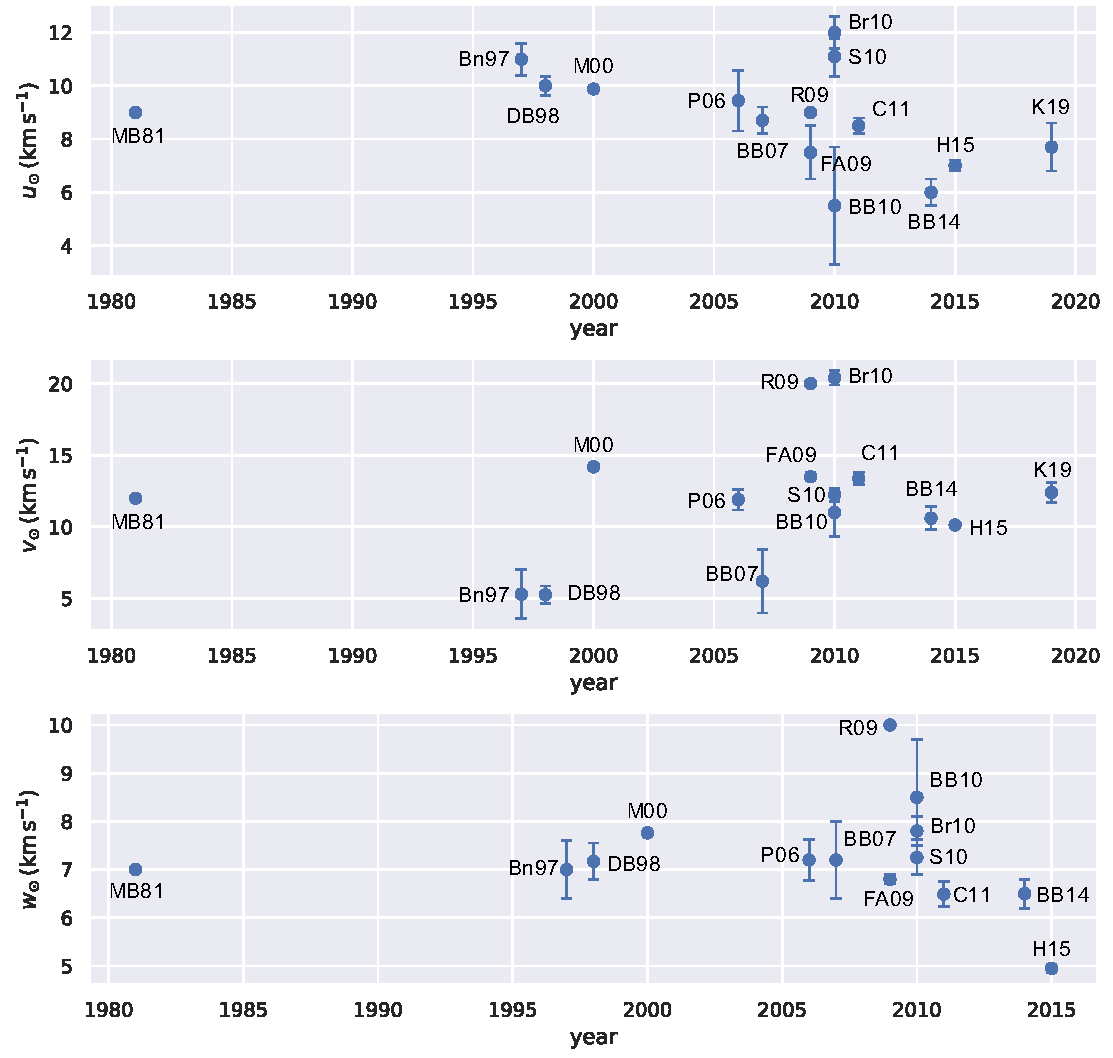
\includegraphics[width=13cm]{fig/UVW.pdf}
	\caption{先行研究の太陽運動の値のプロット。ラベルについては表\ref{table2}を参照。}
	\label{fig:uvw}
\end{figure*}